% ============================================================================
% COURSE REPOSITORY, REMOTE, OVERVIEW
% ============================================================================

\begin{frame}{Course Repository}

\centering
\vspace{0.2cm}
\qrcode[height=3.6cm]{https://github.com/subtilhugo/uzh-llm-socsci-2026}

\vspace{0.5cm}
{\large \href{https://github.com/subtilhugo/uzh-llm-socsci-2026}{\texttt{github.com/subtilhugo/uzh-llm-socsci-2026}}}

\vspace{0.4cm}
{\small New today, in \texttt{sessions/03/}: the notebook, the worksheet, and prompts 10 and 11 in \texttt{template/prompts/}.}

\end{frame}

\begin{frame}{Today, on Zoom}

\begin{itemize}
    \setlength{\itemsep}{8pt}
    \item \textbf{Two windows}: Zoom, and your notebook (Colab or your laptop). The slides are in the repository.
    \item \textbf{Stuck for more than two minutes?} Write in the Zoom chat, then share your screen when I call your name. Someone else is stuck on the same thing.
    \item \textbf{The shared document} is where your numbers go: one line each, at each ``We check''.
    \item \textbf{Keys}: paste them in Colab Secrets or in \texttt{.env}. Never in the chat, never on a shared screen.
    \item \textbf{Camera on during ``We check''} if you can. It is a workshop.
\end{itemize}

\end{frame}

\begin{frame}{Today's Session Overview (9:00--12:00)}

\setlength{\leftmargini}{2.3cm}
\small
\begin{enumerate}
    \setlength{\itemsep}{1pt}
    \item[\textbf{9:00--9:15}] Last Week, and Today's Question {\footnotesize (15 min)}

    \item[\textbf{9:15--10:00}] Part 1. APIs: What They Are, How to Collect from One {\footnotesize (45 min)}
    \begin{itemize}
        \item Requests, keys, limits, versions; the Manifesto Project; is the collection complete?
    \end{itemize}

    \item[\textbf{10:00--10:45}] Part 2. Annotating Through an LLM API {\footnotesize (45 min)}
    \begin{itemize}
        \item You code 15 sentences, then Claude codes 200; you, the coders and the model
    \end{itemize}

    \item[\textbf{10:45--10:55}] Break

    \item[\textbf{10:55--11:30}] Part 3. A Model on Your Own Machine {\footnotesize (35 min)}
    \begin{itemize}
        \item Ollama, and the alternatives; the same task, the same code
    \end{itemize}

    \item[\textbf{11:30--11:50}] Part 4. The UZH ScienceCluster {\footnotesize (20 min, demo)}
    \begin{itemize}
        \item Three doors: the terminal, an agent, the browser
    \end{itemize}

    \item[\textbf{11:50--12:00}] Debrief and Next Session
\end{enumerate}

\end{frame}

% ============================================================================
% LAST WEEK
% ============================================================================

\sectionslide{Last Week}{What we saw, and the question we left open}

\begin{frame}{Last Week, in One Slide}

\small
\textbf{The method.} Document, then specify, then implement, then review, then audit by hand (prompts 06 to 09). The agent writes scripts, never numbers in a chat.

\vspace{0.25cm}

\textbf{The checks.} Row counts at every step, assertions that stop the script, cross-tabulations after every recode and merge.

\vspace{0.25cm}

\textbf{The lesson.} The agent took decisions alone on your data. Finding them was the point.

\vspace{0.5cm}

\textbf{The question we left open}

\vspace{0.15cm}
\centering
\alert{An API returns 10,000 documents and the agent reports\\ that the collection is complete. How would you know?}

\vspace{0.2cm}
{\small Keep your answer in mind. We answer it in Part 1, with real data.}

\end{frame}

\begin{frame}{Today's Thread: One Dataset, Three Coders}

\small
\textbf{The data.} French party manifestos, split into quasi-sentences and coded by trained human coders of the Manifesto Project. We download them through an API.

\vspace{0.3cm}

\textbf{The task.} Assign each quasi-sentence to a policy domain: the economy, welfare, the fabric of society, \dots

\vspace{0.3cm}

\textbf{Three coders, and you}
\begin{itemize}
    \setlength{\itemsep}{2pt}
    \item The Manifesto Project's human coders: our benchmark, not the truth
    \item Claude, through an API: a large commercial model, paid per token
    \item A model on your own machine: open weights, free per call, nothing leaves your laptop
    \item You: 15 sentences, coded before you see any model output
\end{itemize}

\vspace{0.3cm}

\textbf{The question for your project.} When can you put a model's labels in a paper, and what do you have to show?

\end{frame}

% ============================================================================
% PART 1: APIs
% ============================================================================

\sectionslide{Part 1. APIs}{What they are, and how to collect from one}

\begin{frame}{What an API Is}

\centering
\begin{tikzpicture}[font=\small,node distance=1cm]
  \node[draw,rounded corners,fill=gray!15,minimum height=1.2cm,minimum width=2.6cm,align=center] (you) {Your script};
  \node[draw,rounded corners,fill=titleblue!70,text=white,minimum height=1.2cm,minimum width=2.6cm,align=center,right=5.6cm of you] (srv) {The provider's\\server};
  \draw[-{Latex},thick] ([yshift=0.25cm]you.east) -- node[above,font=\scriptsize]{request: URL + parameters + key} ([yshift=0.25cm]srv.west);
  \draw[-{Latex},thick] ([yshift=-0.25cm]srv.west) -- node[below,font=\scriptsize]{response: status code + JSON} ([yshift=-0.25cm]you.east);
\end{tikzpicture}

\vspace{0.5cm}
\raggedright
\begin{itemize}
    \setlength{\itemsep}{5pt}
    \item \textbf{An application programming interface} is a door the provider built on purpose, for programs rather than for people.
    \item \textbf{Compared to scraping a website}: the format is documented and stable, the data are versioned, and the rules are written down (key, limits, licence).
    \item \textbf{Everything today is an API}: the Manifesto Project at 9:30, Claude at 10:15, the model on your laptop at 11:00 (it answers on \texttt{localhost}).
\end{itemize}

\end{frame}

\begin{frame}[fragile]{Anatomy of a Request}

\centering
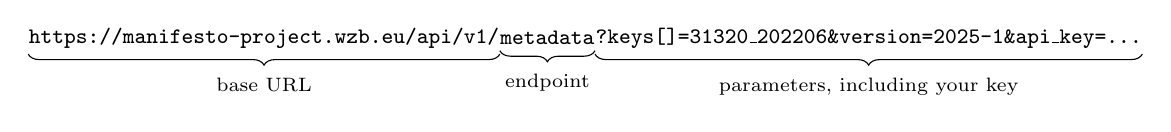
\begin{tikzpicture}[font=\footnotesize\ttfamily]
  \node[anchor=west,inner sep=0] (a) at (0,0) {https://manifesto-project.wzb.eu/api/v1/};
  \node[anchor=west,inner sep=0] (b) at (a.east) {metadata};
  \node[anchor=west,inner sep=0] (c) at (b.east) {?keys[]=31320\_202206\&version=2025-1\&api\_key=...};
  \draw[decorate,decoration={brace,mirror,amplitude=4pt}] ([yshift=-2pt]a.south west) -- node[below=5pt,font=\scriptsize\rmfamily]{base URL} ([yshift=-2pt]a.south east);
  \draw[decorate,decoration={brace,mirror,amplitude=4pt}] ([yshift=-2pt]b.south west) -- node[below=5pt,font=\scriptsize\rmfamily]{endpoint} ([yshift=-2pt]b.south east);
  \draw[decorate,decoration={brace,mirror,amplitude=4pt}] ([yshift=-2pt]c.south west) -- node[below=5pt,font=\scriptsize\rmfamily]{parameters, including your key} ([yshift=-2pt]c.south east);
\end{tikzpicture}

\vspace{0.3cm}
\raggedright
\begin{columns}[T]
\column{0.42\textwidth}
\small
\textbf{Status codes}

{\footnotesize
\begin{tabular}{@{}ll@{}}
\texttt{200} & fine: read the content \\
\texttt{401}, \texttt{403} & bad or missing key \\
\texttt{404} & wrong endpoint or identifier \\
\texttt{429} & too many requests: wait \\
\texttt{5xx} & server error: wait, retry \\
\end{tabular}}

\column{0.54\textwidth}
\small
\textbf{In Python}

{\scriptsize
\begin{verbatim}
r = requests.get(BASE + "metadata",
        params={"keys[]": keys, "version": "2025-1",
                "api_key": KEY},
        timeout=60)
r.status_code     # 200?
r.json()          # the content
\end{verbatim}}
\end{columns}

\vspace{0.25cm}
{\footnotesize Read four things in every response: the status, the content, what is missing, and the version of the data you got.}

\end{frame}

\begin{frame}{APIs Researchers Use}

\small
\begin{itemize}
    \setlength{\itemsep}{3pt}
    \item \textbf{Party politics}: the Manifesto Project (texts and codes); ParlGov; parliaments' open-data services
    \item \textbf{Official statistics}: INSEE (France), the Swiss Federal Statistical Office, Eurostat, the World Bank
    \item \textbf{Literature}: OpenAlex, Crossref, Semantic Scholar (metadata, citations, abstracts)
    \item \textbf{Media and platforms}: news archives, YouTube, Bluesky; X and Reddit restricted or paid since 2023
    \item \textbf{Models}: every LLM provider, and the model on your laptop
\end{itemize}

\vspace{0.25cm}

\textbf{Before you write a line of code, read three pages of the documentation}
\begin{enumerate}
    \setlength{\itemsep}{2pt}
    \item The terms of use: may you redistribute the data? What must you cite?
    \item The limits: requests per minute, per day; pages of results
    \item The versions: which release, and what changed between releases
\end{enumerate}

\vspace{0.15cm}
{\footnotesize Prompt 10: the agent reads them first, and tells you, before it writes the collector.}

\end{frame}

\begin{frame}{Keys: Five Rules}

\begin{enumerate}
    \setlength{\itemsep}{7pt}
    \item \textbf{Never in the code.} In \texttt{.env} on your laptop, in Colab Secrets in a notebook.
    \item \textbf{Never in git.} \texttt{.env} is in your \texttt{.gitignore} since Session 1. Check: \texttt{git check-ignore .env}.
    \item \textbf{Never on a shared screen}, in a chat, in a prompt to an agent, or in an error message.
    \item \textbf{Cap what a key can spend.} Paid APIs let you set a monthly limit. Today's workshop key has one.
    \item \textbf{Leaked? Revoke it at once}, then make a new one. Bots scan public repositories for keys within minutes.
\end{enumerate}

\vspace{0.35cm}

\centering
{\small A key is a password that spends money or quota. Treat it like one.}

\end{frame}

\begin{frame}{Why a Collection Is Silently Incomplete}

\small
\begin{itemize}
    \setlength{\itemsep}{6pt}
    \item \textbf{Pagination}: the API returns 100 results per page; the script read the first page.
    \item \textbf{Rate limits}: request 412 got a \texttt{429}; the script skipped it and went on.
    \item \textbf{Missing items}: you asked for 12 documents; the answer lists 2 as missing. Nobody read that field.
    \item \textbf{Versions}: the provider corrected the data last month; your colleague downloaded before.
    \item \textbf{Filters you did not choose}: a default language, period or country in the endpoint.
\end{itemize}

\vspace{0.4cm}

\textbf{None of these raises an error.} The script ends; the agent reports success; the data are wrong.

\end{frame}

\begin{frame}{Last Week's Question, Answered}

\small
\textbf{Four checks, written into the collector}

\vspace{0.1cm}
\begin{enumerate}
    \setlength{\itemsep}{5pt}
    \item \textbf{Accounting.} Requested = returned + listed as missing. Nothing silently dropped.
    \item \textbf{Content.} No empty record, no duplicate, every field you need present.
    \item \textbf{A published total.} The provider publishes the number of quasi-sentences of each manifesto in its core dataset. Our count must match it.
    \item \textbf{A published statistic, recomputed.} The core dataset gives each party's share of welfare-expansion statements (\texttt{per504}). Recompute it from the texts.
\end{enumerate}

\vspace{0.2cm}

\textbf{And archive the raw answers} before any processing, with the version and a log of every request. If a check fails in a month, you can find out why.

\vspace{0.2cm}

\centering
\alert{Completeness is checked against a number the provider published independently of your request, not against the agent's report.}

\end{frame}

\begin{frame}{The Manifesto Project}

\small
%%MANIFESTO%%

\end{frame}

\begin{frame}{Block 1. Collect (9:35--10:00)}

\small
\textbf{I show (10 min).} The notebook, Parts 1 and 2: the first request, the French manifestos of one election, the raw answer archived, the four checks.

\vspace{0.3cm}

\textbf{You do (10 min)}
\begin{enumerate}
    \setlength{\itemsep}{3pt}
    \item Open the notebook (\texttt{sessions/03/}, button ``Open in Colab''). Your Manifesto key in Colab Secrets.
    \item Run Parts 1 and 2. Read the four checks before going on.
    \item No key yet? Option B in Part 2 loads the same table from the repository.
    \item Faster than the others: prompt 10 in your own project, on the API you brought.
\end{enumerate}

\vspace{0.3cm}

\textbf{We check (5 min).} The shared document: requested, returned, missing, and the published number you checked against.

\end{frame}

% ============================================================================
% PART 2: ANNOTATION THROUGH AN API
% ============================================================================

\sectionslide{Part 2. Annotating Through an LLM API}{The same door, a different provider}

\begin{frame}{Why Annotate with an LLM}

\footnotesize
\textbf{Why it caught on}
\begin{itemize}
    \setlength{\itemsep}{2pt}
    \item Zero-shot ChatGPT beat crowd workers on four of five tasks, for a fraction of the cost (Gilardi, Alizadeh and Kubli 2023, \textit{PNAS}, here at UZH).
    \item GPT-4 beat expert coders and supervised classifiers on political tweets (T\"ornberg 2025); few-shot prompts matched supervised methods (Ornstein et al.\ 2025).
    \item On manifestos, LLM positions correlate 0.87 to 0.92 with expert surveys (Benoit et al.\ 2026, \textit{AJPS}).
\end{itemize}

\vspace{0.15cm}

\textbf{Why it needs validation}
\begin{itemize}
    \setlength{\itemsep}{2pt}
    \item Zero-shot models do not beat fine-tuned ones at classification (Ziems et al.\ 2024).
    \item Small open models follow codebooks poorly, and worst of all on Manifesto data (Halterman and Keith 2026, \textit{Political Analysis}).
    \item Answers change with the wording of the prompt, and on a simple rerun (Reiss 2023; Barrie, Palaiologou and T\"ornberg 2026).
    \item Labels at 80--90\% accuracy still bias a regression that uses them, unless corrected with a gold sample (Egami et al.\ 2023).
\end{itemize}

\vspace{0.1cm}
\centering
\alert{Cheap labels, expensive validation.}

\end{frame}

\begin{frame}{The Pipeline}

\centering
\begin{tikzpicture}[font=\scriptsize,node distance=0.35cm,scale=0.9,transform shape]
  \tikzset{box/.style={draw,rounded corners,minimum height=0.8cm,align=center,fill=gray!12},
           key/.style={draw,rounded corners,minimum height=0.8cm,align=center,fill=titleblue!70,text=white}}
  \node[box] (cb) {Codebook\\(system prompt)};
  \node[box,below=of cb] (it) {One quasi-sentence\\(+ the previous one)};
  \node[box,below=of it] (sc) {Schema\\(reason, domain)};
  \node[key,right=0.9cm of it,minimum width=1.6cm] (m) {Model};
  \node[box,right=0.7cm of m] (js) {JSON\\answer};
  \node[box,right=0.6cm of js] (log) {\texttt{raw.jsonl}\\every answer kept};
  \node[box,below=0.9cm of log] (val) {Validation\\against humans};
  \draw[-{Latex}] (cb.east) -- (m.west);
  \draw[-{Latex}] (it.east) -- (m.west);
  \draw[-{Latex}] (sc.east) -- (m.west);
  \draw[-{Latex}] (m) -- (js);
  \draw[-{Latex}] (js) -- (log);
  \draw[-{Latex}] (log) -- (val);
  \node[font=\scriptsize,text=gray,below=0.15cm of m,align=center] {once per item,\\200 times};
\end{tikzpicture}

\vspace{0.35cm}
\raggedright
\small
\begin{itemize}
    \setlength{\itemsep}{3pt}
    \item \textbf{The codebook is the method.} It lives in a file, versioned, and goes in your appendix.
    \item \textbf{A schema, not free text.} The model must return valid JSON with one of eight labels: no parsing, no ``I think it is probably\dots''.
    \item \textbf{A reason before the label.} One sentence. You read it when you disagree.
    \item \textbf{Every answer is appended to a file as it arrives.} A crash or a rerun never pays twice.
\end{itemize}

\end{frame}

\begin{frame}[fragile]{One Call, in Code}

\scriptsize
\begin{verbatim}
class Annotation(BaseModel):
    reason: str
    domain: Literal["external_relations", "freedom_democracy", "political_system",
                    "economy", "welfare_quality_of_life", "fabric_of_society",
                    "social_groups", "no_category"]

r = claude.messages.parse(
    model="claude-haiku-5-5",              # a pinned snapshot: report it as is
    max_tokens=300,
    system=[{"type": "text", "text": CODEBOOK,
             "cache_control": {"type": "ephemeral"}}],   # same codebook: cached
    messages=[{"role": "user", "content": "PREVIOUS: ...\nTARGET: ..."}],
    output_format=Annotation,              # the answer must fit the schema
    thinking={"type": "disabled"},         # a short task: no thinking
)
r.parsed_output.domain, r.parsed_output.reason, r.usage
\end{verbatim}

\vspace{0.2cm}
\small
Read the whole response once, before you run 200: \texttt{stop\_reason}, \texttt{usage}, the model that answered.

\end{frame}

\begin{frame}{What It Costs}

\small
\textbf{Prices per million tokens, input / output} {\footnotesize (official pages, 3 November 2026)}

\vspace{0.1cm}
\centering
{\footnotesize
\renewcommand{\arraystretch}{1.1}
\begin{tabular}{@{}llll@{}}
\toprule
\textbf{Model} & \textbf{Provider} & \textbf{Price} & \textbf{Note} \\
\midrule
Claude Haiku 5.5 & Anthropic & \$0.10 / \$0.50 & today; cache hits \$0.01 \\
Claude Sonnet 5.5 & Anthropic & \$2 / \$10 & 20 times more \\
GPT-6 Luna & OpenAI & \$0.10 / \$0.50 & reasoning model \\
Gemini 3.5 Flash-Lite & Google & \$0.30 / \$2.50 & free tier exists \\
Mistral Small 4 & Mistral (EU) & \$0.15 / \$0.60 & open weights, Apache 2.0 \\
A model on your laptop & you & \$0 per call & your time, your hardware \\
\bottomrule
\end{tabular}}

\vspace{0.3cm}
\raggedright
\begin{itemize}
    \setlength{\itemsep}{3pt}
    \item \textbf{Our 200 sentences}: a few hundred tokens of codebook (cached after the first call), about 60 of text and 30 of answer each. \textbf{Under two cents.} The notebook prints the real figure.
    \item \textbf{Batch APIs} halve the price, for answers within 24 hours: the way to code a whole corpus.
    \item \textbf{Free tiers} (Google, Mistral) may use your data to train their models; in Switzerland and the EU, Google applies its paid terms. Read the terms before sending research data.
\end{itemize}

\end{frame}

\begin{frame}{Reproducibility with a Closed Model}

\small
\begin{itemize}
    \setlength{\itemsep}{6pt}
    \item \textbf{Pin the model.} \texttt{claude-haiku-5-5} names one snapshot; Anthropic does not change its weights. Report the ID, never ``Claude''.
    \item \textbf{You cannot fix the randomness.} The current Claude models do not accept \texttt{temperature}; OpenAI's reasoning models neither, and its \texttt{seed} is deprecated. So: run twice, and report how many answers change.
    \item \textbf{The serving can still change}, even with the same weights; and a model ID is retired one day. Your archived answers are the record, not the model.
    \item \textbf{Archive everything}: the prompt file, the schema, the parameters, every raw answer, the date. That is the reproducibility bundle of Session 2, in Part 7 of the notebook.
    \item \textbf{The model may have seen your data.} Manifestos are on the web; the model may have read them, and even their codes, in training. A held-out or new corpus is the honest test.
\end{itemize}

\end{frame}

\begin{frame}{Validation: Four Numbers, Not One}

\small
\begin{enumerate}
    \setlength{\itemsep}{6pt}
    \item \textbf{Agreement with careful human coding}: accuracy, macro-F1, Cohen's $\kappa$ (agreement corrected for chance). Read the confusion matrix, not only the number.
    \item \textbf{Stability}: the same items, a second run. How many answers change?
    \item \textbf{Your own agreement with the coders}, on 15 sentences. If you agree with them only 60\% of the time, a model at 70\% is not bad: the task is hard.
    \item \textbf{The aggregate your paper reports}: each party's share of welfare statements, computed from the coders and from the model. Sentence-level errors can cancel out, or pile up in one direction.
\end{enumerate}

\vspace{0.3cm}

%%HUMANREL%%

\end{frame}

\begin{frame}{Block 2. Annotate (10:15--10:45)}

\small
\textbf{I show (5 min).} Part 3: the seven domains and the sample. Part 4: one call, read in full, then 200.

\vspace{0.3cm}

\textbf{You do (20 min)}
\begin{enumerate}
    \setlength{\itemsep}{3pt}
    \item \textbf{Code your 15 sentences first} (Part 3), before any model output. Ten minutes.
    \item Your Anthropic key (the workshop key, in the email) in Colab Secrets. Part 4: one call, then the 200.
    \item Part 6, first three cells: the scores, your agreement, the confusion matrix.
    \item Read five disagreements. Who is right, the coder or the model?
\end{enumerate}

\vspace{0.3cm}

\textbf{We check (5 min).} The shared document: your agreement with the coders, the model's $\kappa$, and one sentence where you think the model is right.

\end{frame}

\begin{frame}[plain]
  \centering
  \vfill
  {\LARGE \textbf{\textcolor{titleblue}{Break}}}\\[0.4cm]
  {\large 10:45 -- 10:55}\\[0.6cm]
  {\small Laptop users: start \texttt{ollama pull %%PULLMODEL%%} now if you did not last night.}
  \vfill
\end{frame}
